%# -*- coding: utf-8-unix -*-
%%==================================================
%% chapter_4.tex for SJTU Master Thesis
%%==================================================

\chapter{伺服系统设计及统计策略拓展应用及仿真}
在本章中,首先将从时钟伺服角度进行分析,并采用相关PID控制算法来提高从时钟系统稳定性。另外,为了能够计算得到准确的offset,还将通过对从时钟晶振频率进行补偿以使得主从时钟频率尽可能保持一致来消除offset波动所带来的问题。其次,本章节还将介绍如何将稳中提到的统计算法应用到透明时钟中,由于透明时钟与边界时钟的根本差异,需要对统计算法进行调整才能更好的应用到透明时钟中。最后,本节将对文中采用的算法进行仿真,并对仿真结果进行分析总结。

\section{时钟伺服系统研究}
在第\ref{chap:statistical_delay}章中,从链路传输延时的角度,通过深入分析实际工业环境下对链路传输延时的影响,通过对链路传输延时建立细致的数学模型,并从数学统计的角度对其中各个影响因素采用了有针对性的解决方案。至此,已经能够利用上述算法综合获得稳定和精确的链路延时。但是,仅仅获取稳定精确的链路延时并不是时钟同步的终点。而且,在现实IEEE1588协议运行中,之所以同步精度难以达到亚微秒的同步精度,有很重要的因素是从时钟校正策略的选取。所谓时钟同步,最核心一环自然是从时钟根据计算数据对本地进行校正来实现同步,即时钟伺服系统。常规上在IEEE1588协议中采用的是PI控制策略,即利用PI控制器来对从时钟进行校正,而不是直接利用offset进行校正。这种做法能够一定程度提高从时钟的同步精度和稳定性,但它也存在如PI参数固定等缺陷而导致同步系统无法有效应对复杂多变的工业网络环境,这严重破坏了从时钟系统的稳定性。另外,想要提高同步精度意味着必须得出准确的主从偏差值offset,并对从时钟进行校正。但是,主从偏差值会由于晶振源频率波动而变化,所以依据常规的同步算法并不能消除这个问题。

对从时钟而言,如果想要实现与主时钟同步,就必须依靠前面提到的同步算法及所计算出来的链路时延值,从而对从时钟自身的相位和频率进行校正,以有效消除与主时钟之间的偏差。不过,由于当前的很多工业平台并非实时操作系统,所以一般而言都需要利用中断机制来触发从时钟进行校正。但是,在该中断过程中造成的从时钟漂移抖动会长期破坏同步精度,严重影响同步过程的实时性。

因此,为了提高从时钟校正过程的实时性和快速性,需要设计一套比较良好的时钟伺服系统来对从时钟进行校正。

\subsection{通用PTP时钟伺服系统介绍}
\begin{figure}[hbp]
  \centering
  \begin{minipage}[b]{0.7\textwidth}
   \captionstyle{\centering}
   \centering
   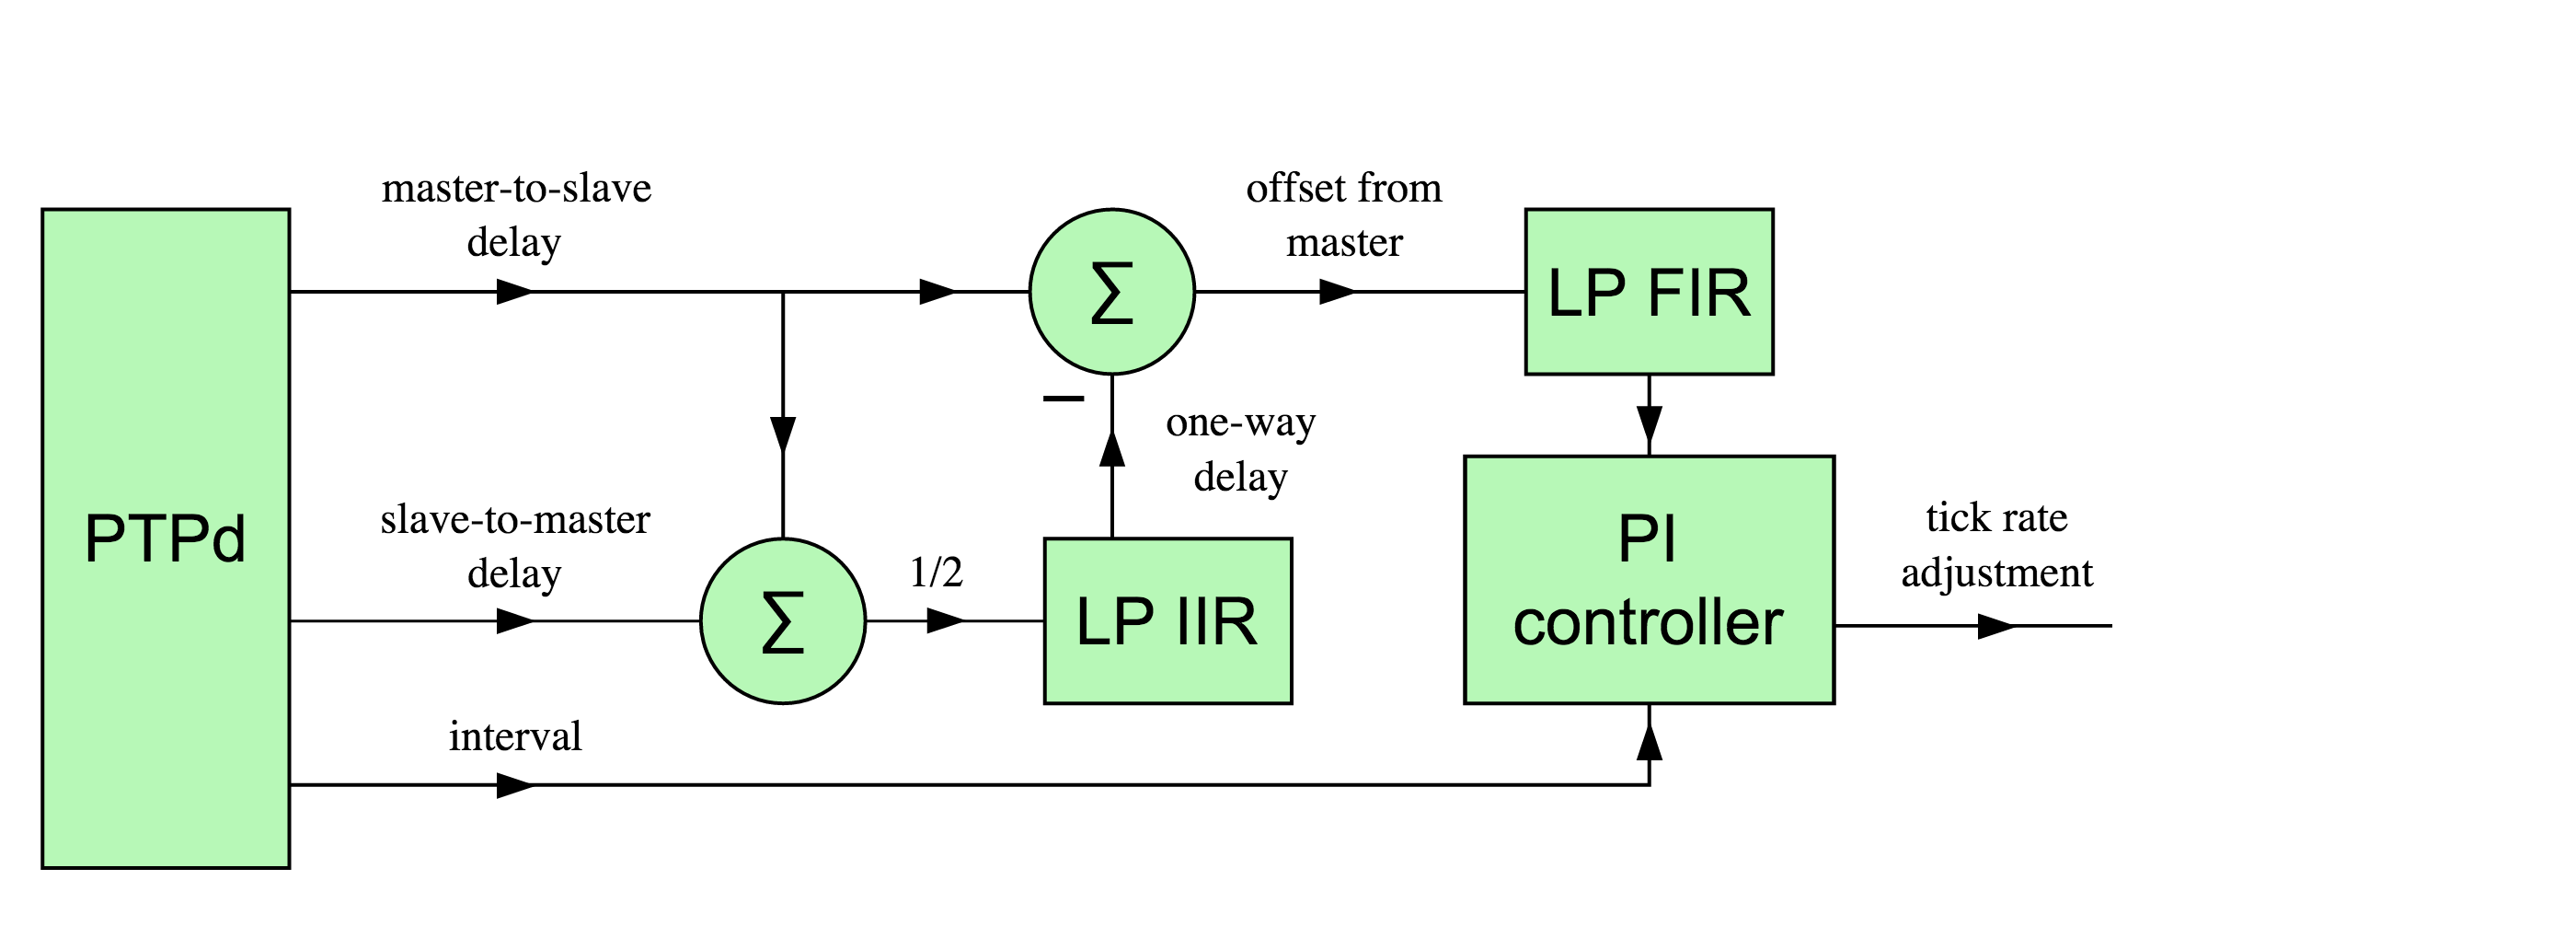
\includegraphics[width=11cm]{normal_clock_servo_system}
   \bicaption[fig:normal_clock_servo_system]{通用PTP时钟伺服系统}{通用PTP时钟伺服系统}{Fig}{The normal structure of general PTP clock servo system}
  \end{minipage}
\end{figure}

一种常见的PTP时钟伺服系统如图\ref{fig:normal_clock_servo_system}所示\supercite{58}。从左到右表明了数据从PTP协议引擎逐渐流向从时钟。在该系统中,PTP协议引擎通过周期性获取主从偏差和从主偏差,将这两个偏差值通过均值滤波及低通滤波器获取到当前offset值。然后,将当前offset值与采样周期数据共同传递给PI控制器,由PI控制器来对从时钟进行校正以实现主从同步。该PI控制器由比例(P)和积分(I)两个环节共同构成,其中,比例环节可以用来消除主从时钟间的相位偏差,而积分项则可以用来消除系统的稳态误差,即消除主从时钟间的频率差\supercite{58}。

上述这样一套较为完整的时钟伺服系统可以较好的实现时钟同步,而且,PID控制器由于具有算法简单、鲁棒性好和可靠性高等特点,在实际控制系统设备中得到广泛的运用,而且PI控制是在工业过程控制中应用最为广泛的一种控制算法。

下文将从PID控制角度出发,结合同步系统特性进行深入分析,并且将基于第三章中统计算法得到的样本值来对控制器进行调整,从而来弥补传统PID控制器无法适应复杂网络环境的缺陷。

PID控制器的基本结构由比例单元P、积分单元I和微分单元D组成。透过Kp,Ki和Kd三个参数的设定。PID控制器主要适用于线性且动态特性不时变的系统。它是工业控制应用中常见反馈回路部件,会把收集的数据与一个参考值比较,并把该差值用于新的输入值计算中,这个新输入值的目的是让系统数据达到或者保持在参考值。另外,它还可以根据历史数据来调整输入值以提高系统准确度和稳定度。

PID控制器中含有比例单元P、积分单元I和微分单元D,它们分别对应目前误差、历史累计误差及未来误差。在不清楚受控系统特性的情况下,一般认为PID控制器是最适用的控制器。它可以通过调整PID三个参数来调整控制系统以满足设计需求。然后可以用控制器对误差的反应快慢、控制器过冲程度及系统震荡来表示控制器反应程度。

% \begin{figure}[!hbp]
%   \centering
%   \begin{minipage}[b]{0.7\textwidth}
%    \captionstyle{\centering}
%    \centering
%    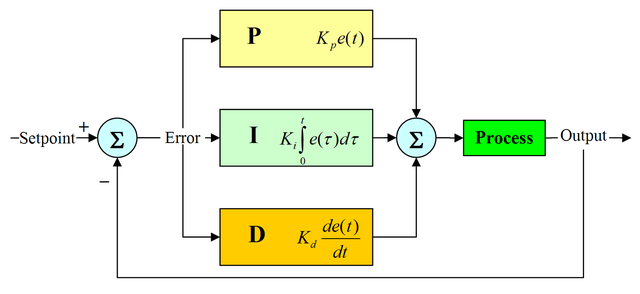
\includegraphics[width=11cm]{pid_controller.png}
%    \bicaption[fig:pid_controller]{PID控制器结构}{PID控制器结构}{Fig}{The normal structure of PID controller}
%   \end{minipage}     
% \end{figure}

\subsection{基于统计算法的PID控制器设计}
第三章中采用的统计算法是通过在从时钟处累计PTP报文及链路延时样本,通过滤波、阈值限制与动态监控方法以提高链路延时精确度,从而得到更为精确的链路延时数据样本。不过,如果直接拿计算得到的主从偏差去进行从时钟校正,那么很有可能会破坏从时钟的稳定性。

所谓时钟同步,希望达到的目的是主从时钟的时间差趋于零,从而使得主从时钟保持一致。而且,在这个一致的过程中,不仅仅希望从时钟能与主时钟的偏差很小,更希望从时钟的波动很小,即具备良好的稳定性,同时,一旦链路中发生波动的因素,也希望从时钟能够不会产生明显的波动,即具备良好的鲁棒性。

所以,为了提高同步系统的稳定性和鲁棒性,这里采用了PID控制器,来对整个同步系统进行控制,以保证从时钟的稳定性和鲁棒性。假设控制器的输入偏差为Error(t),对应的控制器输出为Output(t),那么根据PID控制器原理,可以得到如下计算公式:
\begin {align}
Output(k) = K_{p} * Error(k) + K_{i} * \sum_{i=1}^{k}Error(i) + K_{d}\Delta Error(k)
\end{align}
\begin {align}
Output(k) = K_{p} * [\frac{1}{T_{d}} * \sum_{0}^{k}Error(i) + T_{d} * \frac{dError(t)}{dt}]
\end{align}
\begin {align}
\Delta Output(k) = K_{p}(E(k) - E(k-1)) + K_{i}E(k) + K_{d}(E(k) - 2E(k-1) + E(k-2))
\end{align}
\begin {align}
\Delta Output(k) = Output(k) - Output(k-1)
\end{align}
其中,Error(k)为主从时间偏差。希望达到的目的是使的Error(k)趋近于零,也就是使的主从时间差尽可能小。这里采用公式(4-3)来进行分析,假设当前时刻为k,那么可以通过Error(k)、Error(k-1)、Error(k-2)来计算得出当前的控制量$\Delta Output(k)$。所以,为了获取当前控制量,必须获得连续三个主从偏差值offset。

根据上面可以知道,通过三个连续偏差值Error(k)、Error(k-1)、Error(k-2),结合PID控制器可以计算出所需要的控制量,将该控制量作用于从时钟即可达到时钟同步的效果。如图\ref{fig:time-window-pid}。
\begin{figure}[htbp]
  \centering
  \begin{minipage}[b]{0.7\textwidth}
   \captionstyle{\centering}
   \centering
   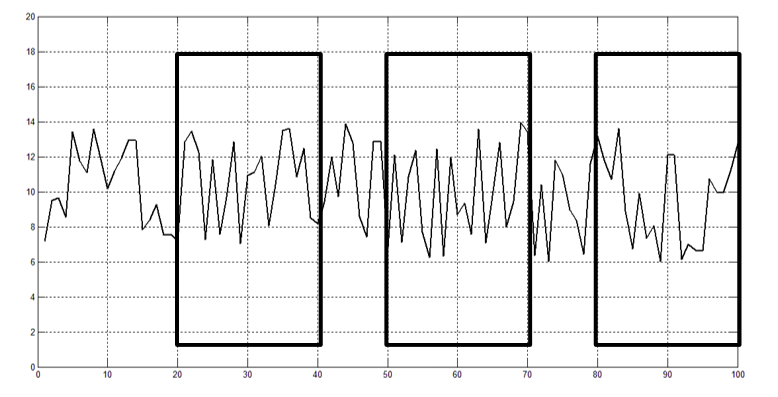
\includegraphics[width=11cm]{time-window-pid.png}
   \bicaption[fig:time-window-pid]{时间窗连续取值}{时间窗连续取值}{Fig}{The time-window value figure}
  \end{minipage}     
\end{figure}


那么,这里存在一个问题,就是如果链路延时发生了阶跃变化,如果继续使用常规的PID控制,那么可能会导致控制量出现较大的变化,从而引发从时钟的不稳定。可以参考图\ref{fig:sliding-window-pid},使用一个长度为十的滑动时间窗来获取上面的连续偏差值,当发生阶跃变化时,滑动窗内的取值也会发生较大的波动,不过,对于这种阶跃变化,最初时无法判断是暂时性突变还是持久性变化,所以,为了保证从时钟的稳定性,这里要调整控制结构。
\begin{figure}[htbp]
  \centering
  \begin{minipage}[b]{0.7\textwidth}
   \captionstyle{\centering}
   \centering
   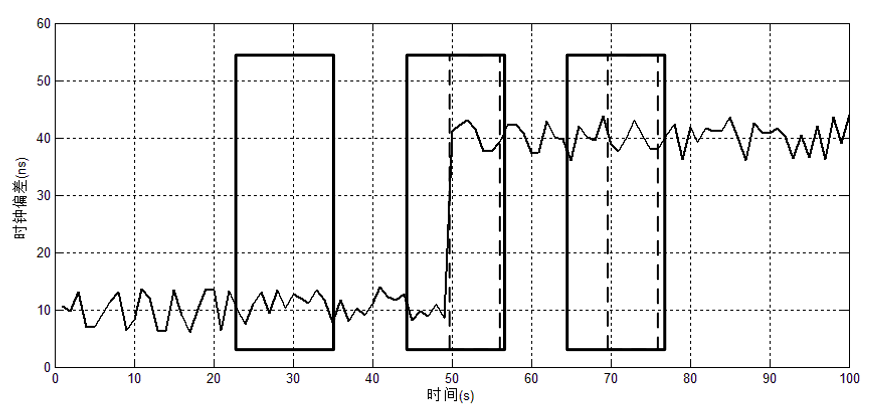
\includegraphics[width=11cm]{sliding-window-pid.png}
   \bicaption[fig:sliding-window-pid]{滑动时间窗阶跃检测}{滑动时间窗阶跃检测}{Fig}{The sliding-window step-signal detection figure}
  \end{minipage}     
\end{figure}

因此,本文采用一种多模型PID控制系统,即通过检测主从时间偏差的变化情况来选择合适的控制器,从而保证从时钟能达到尽可能的稳定。

具体的结构如图\ref{fig:multi-model-servo}。
\begin{figure}[htbp]
  \centering
  \begin{minipage}[b]{0.7\textwidth}
   \captionstyle{\centering}
   \centering
   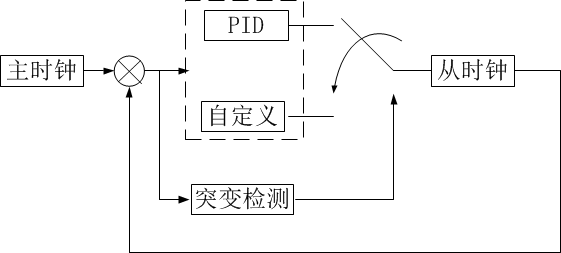
\includegraphics[width=11cm]{multi-model-servo.png}
   \bicaption[fig:multi-model-servo]{基于多模型PID控制器结构}{基于多模型PID控制器结构}{Fig}{The multi-model PID controller}
  \end{minipage}     
\end{figure}

其中的原理是,在控制器前面,采用突变检测器,判断误差是否发生了阶跃性变化,如果没发生则使用正常的PID控制器;一旦检测发现阶跃性变化发生,则暂时使用自定义控制环节,保持偏差量不变,去对从时钟进行校正。同时继续等待一段时间,这段时间可以根据经验法去获取,如果误差重新发生阶跃性恢复到原始状态或者稳定不变,那么就继续使用PID控制器。

其中,突变检测器就是用来监测残差信号是否发生阶跃性变化,具体的方法类似上一章节中的动态阈值法,通过在一定的时间窗内观测信号的变化情况,我们取时间窗长度为十,如果发现当前信号处于突变中,那就切换控制模型,从PID控制模型切换到下列模型:
\begin {align}
u(k) = u(k-1)
\end{align}
也就是使用历史数据来替代当前突变数据,从而保持从时钟的稳定性。当时间窗继续向前滑动,信号的抖动逐渐恢复。则可以恢复使用PID控制器来进行控制。

\subsection{多模型PID控制器仿真及分析}
首先,这里先对PID参数进行整定。所谓PID参数整定就是确定调节器的比例常数$K_{p}$、$K_{i}$、$K_{d}$,一般而言,可以采用理论计算来进行参数整定,但是一般误差比较大。在当前工业实际中,较多的是采用工程整定法,例如经验法、衰减曲线法、临街比例带法和反应曲线法等等。这里采用经验试凑法来进行PID参数整定。首先,给定$K_{p}$、$K_{i}$参数之,通过改变链路延时添加扰动,以观察控制曲线的形状,同时对$K_{p}$、$K_{i}$进行调整直到同步曲线达到良好的同步效果;然后,在前面整定好的基础上再来调节$K_{d}$微分参数,由于$K_{d}$会抵制偏差变化,所以我们可以稍微减小$K_{p}$、$K_{i}$然后继续调整到最佳值。

经过了上面一步可以把PID控制参数整定好,然后,为了仿真上文采用的多模型PID控制系统方法,我们在链路延时中添加一个阶跃性变化量,同时对常规PID控制和多模型PID控制系统进行比较。

\begin{figure}[htbp]
  \centering
  \begin{minipage}[b]{0.7\textwidth}
   \captionstyle{\centering}
   \centering
   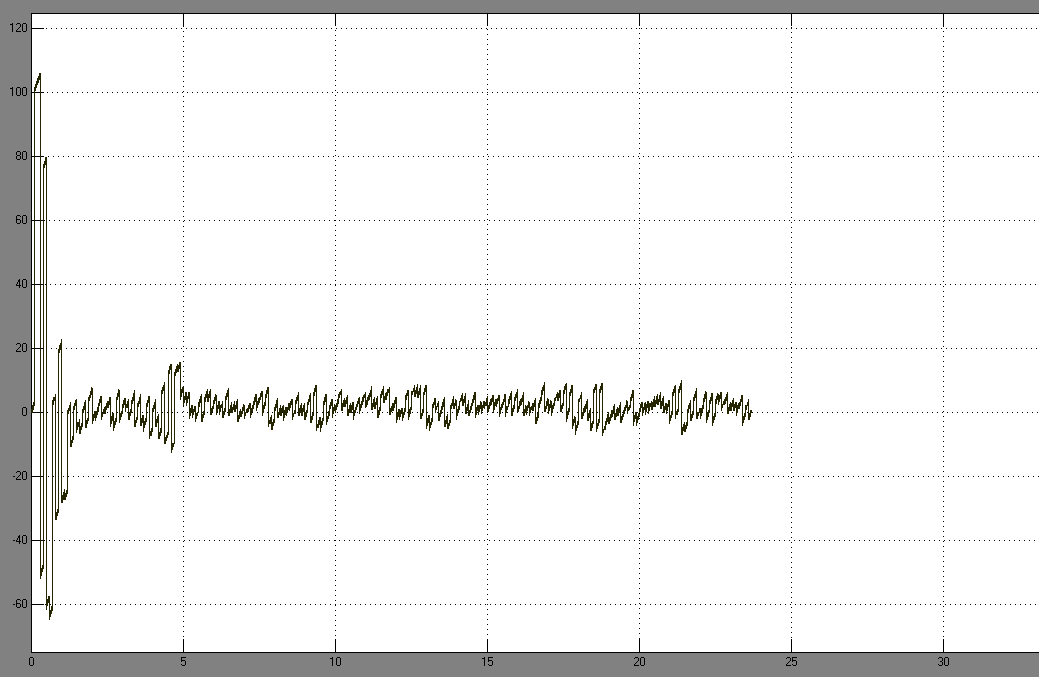
\includegraphics[width=11cm]{matlab/常规PID应对阶跃变化的同步曲线.PNG}
   \bicaption[fig:step_signal_into_normal_pid]{常规PID控制时延突变的同步曲线}{常规PID控制时延突变的同步曲线}{Fig}{The normal PID controller handling step signal of time-delay}
  \end{minipage}     
\end{figure}

\begin{figure}[htbp]
  \centering
  \begin{minipage}[b]{0.7\textwidth}
   \captionstyle{\centering}
   \centering
   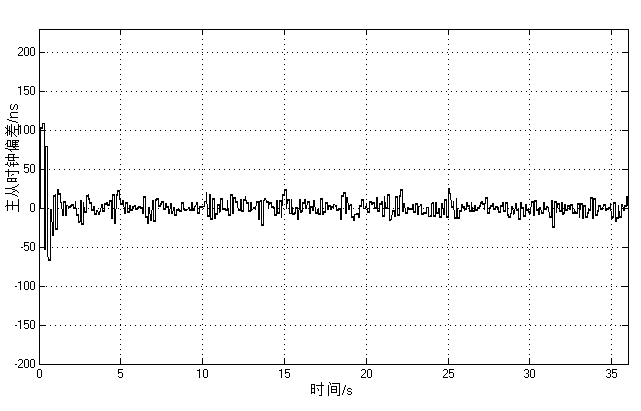
\includegraphics[width=11cm]{matlab/多模型PID应对阶跃变化的同步曲线.PNG}
   \bicaption[fig:step_signal_into_multi_model_pid]{多模型PID应对阶跃变化的同步曲线}{多模型PID应对阶跃变化的同步曲线}{Fig}{The multi-model PID controller handling step signal of time-delay}
  \end{minipage}     
\end{figure}

通过比较上面两个仿真曲线,可以看出,当使用多模型PID控制系统后,对于阶跃突变信号有更好的适应性,从时钟也具有更好的稳定性。

为了提高从时钟的稳定性,常规的做法是直接使用计算误差offset值对从时钟进行校正,不过那种做法会使得从时钟具有较大的波动,而且不能有效利用历史数据来进行调节。因此,本小结首先阐述了时钟伺服系统的概念,使用时钟伺服系统一般能够较好的提高同步系统的稳定性。然后,文中使用常规PID控制器进行校正,不过,为了应对延时阶跃性突变这种情况,文中又采用了一种多模型PID控制系统,即通过对控制误差进行检测,一旦发现控制误差发生阶跃变化,就切换控制器,以防止从时钟发生较大抖动,同时,在一定的观察时间段内,如果控制误差阶跃性恢复到原始值,则立即切换回常规PID控制,否则,直到观测时间短结束,才切回常规PID控制。阶跃信号会使得常规PID控制器控制后的从时钟发生频繁的调整,这会影响到依赖它的整个系统的抖动。而采用多模型PID控制系统可以把持续的波动转变成一个瞬时性的变化,这可以明显减小从时钟的频繁抖动,使整个系统更加稳定。

\section{统计策略在晶振源漂移补偿中的应用研究}
由于在工业现场中采用的ptp时钟设备内部都是通过晶振来计时的,或者说内部时钟就是通过晶振的计数来实现的。然后,晶振本身物理特性比较复杂,一般用以下两个属性来进行描述:准确度和稳定度。其中准确度指系统误差,稳定度指随机误差。在1588同步协议中,晶振频率频偏都会影响到时钟的同步精度。IEEE1588协议中假设在一次同步周期中,主从时钟的偏差会保持不变。然而实际上,虽然主时钟采用高稳时钟,稳定性较高,但是从时钟采用普通晶体振荡器,这使得从时钟频率与标准频率相比存在漂移,也就造成了主从时钟偏差一直处于变化中,也就是说,真实的情况并不满足协议中假设的那样主从偏差保持不变。

因此,由于由于从时钟晶振源的自身漂移,导致了主从时钟之间的偏差处于不断变化中。所以,应该采取手段来补偿从时钟晶振源的漂移,使得主从时钟晶振源保持一致,从而尽可能减小晶振源漂移造成的误差。

\subsection{晶振漂移对1588同步精度的影响}
由于晶振源的精度会同时受到外部环境和内部因素的共同影响,所以实际对外的输出频率是不断变化的。用$f_{output}$表示晶振源对外输出的频率,$f_{standard}$表示标称频率,D表示频率漂移程度,那么可以得到:
\begin {align}
D = \frac{f_{output} - f_{standard}}{f_{standard}}
\end{align}
而在真实的ptp同步系统中,由于主时钟一般采用高稳时钟,所以可以认为主时钟的漂移非常小以至可以忽略,那么假设主从时钟频率漂移为$f_{delta}$,计算方式如下:
\begin {align}
f_{delta} = D * f_{standard}
\end{align}
也就是说,假设一次同步周期为$T_{sync}$,则一次sync过程中主从时钟源的固有漂移值为:
\begin {align}
T_{delta} = D * \frac{f_{delta} * T_{sync}}{f_{standard}}
\end{align}
其中,$T_{delta}$就是一次同步周期内最大的时钟漂移。随着时间的流逝,这种漂移不会不会改善,而且会使得主从晶振源频率漂移越来越大,造成了漂移时间也越来越大,严重破坏了同步精度。

因此,必须对从时钟晶振漂移进行合适的补偿,使得每次同步周期中,从时钟的频率能够进一步靠近主时钟,从而减小频率漂移带来的不良影响。

\subsection{统计算法在频率补偿中的应用}
为了补偿从时钟频率,需要通过一种手段来测量主从时间的频率差值。这里采用的方法就是利用Sync报文的周期性发送,即主时钟是每隔$T_{m}$时间段发送一次Sync报文,而从时钟也是每隔$T_{s}$时间段收到一次Sync报文,假设主从时钟的频率是一致的,那么$T_{m}$就应该接近于$T_{s}$。然而实际上,由于从时钟频率漂移,使得从时钟的计数方式收到影响,导致$T_{s}$并不等于$T_{m}$,不过,正好可以利用这个特性来估算主从时钟的频率差值。

不过,要注意的是,$T_{m}$与$T_{s}$不完全相等并不一定是从时钟漂移所带来的,还有可能是链路上传输的时间波动,导致Sync报文的发送和接收周期不一致。所以,不可以仅仅根据一次Sync报文的发送、接收周期来计算频率差值。针对这样的情况,下文采用了一种基于统计算法的频率补偿方法,下面进行详细介绍:

由于在上面的统计算法中,累积了很多的sync报文样本,可以利用这些sync报文来进行统计分析。
\begin{table}[htpb]
  \centering
  \bicaption[tab:dynamic_threshold]{sync报文收发时间戳}{sync报文收发时间戳}{Table}{Timestamp for send and receive of sync message}
  \begin{tabular}{llllll} \toprule
    sync次序 & 1 & 2 & 3 & $\cdots$ & n \\ \midrule
    当前sync报文发送时间 & $t_{s1}$ & $t_{s2}$ & $t_{s3}$ & $\cdots$ & $t_{sn}$ \\ \midrule
    当前sync报文接收时间 & $t_{r1}$ & $t_{r2}$ & $t_{r3}$ & $\cdots$ & $t_{rn}$  \\ \bottomrule
  \end{tabular}
\end{table}

上面的表格可以很容易通过之前的样本数据得到,有了每个sync报文的发送接收时间后,可以很简单的计算出sync报文的发送接收周期波动值。
\begin{table}[htpb]
  \centering
  \bicaption[tab:dynamic_threshold]{sync报文收发周期}{sync报文收发周期}{Table}{Loop for send and receive of sync message}
  \begin{tabular}{llllll} \toprule
    编号 & 1 & 2 & 3 & $\cdots$ & n \\ \midrule
    sync报文主时钟发送周期 & $T_{m1}$ & $T_{m2}$ & $T_{m3}$ & $\cdots$ & $T_{mn}$ \\ \midrule
    sync报文从时钟接收周期 & $T_{s1}$ & $T_{s2}$ & $T_{s3}$ & $\cdots$ & $T_{sn}$  \\ \bottomrule
  \end{tabular}
\end{table}

因此,能够得到主从时钟的周期样本,利用这些样本,可以采用均值法来计算主从时钟的周期,设主时钟平均周期为$T_{m}$,从时钟平均周期为$T_{s}$,那么可以得到主从时钟频率偏差为:
\begin {align}
f_{delta} = \frac{1}{T_{m}} - \frac{1}{T_{s}}
\end{align}
利用$f_{delta}$即可对从时钟频率进行校正。

除此之外,我们可以对Sync报文采用上一章节中采用的动态监控算法,如果发现该时间段内的Sync报文发生暂时性时延突变,那么意味着内部的Sync报文传输时间会发生突变,那么我们可以选择“抛弃”这个时间段内的Sync报文,等到报文稳定传输后,再去计算频率差值。

\section{统计算法在透明时钟中的应用}
透明时钟是一种新的ptp设备类型,虽然它应用范围不如边界时钟更广,而且其本身需要成本更高,不过为了算法完整性,文中决定对于这类设备的同步优化进行分析。下面的分析主要针对透明时钟与边界时钟的差异性,来分析四种算法暂时性时延抖动优化算法,持久性时延变化优化算法,时延固有波动优化算法和主从时钟源频率补偿算法的调整。

\subsection{透明时钟与边界时钟差异性}
透明时钟(Transparent Clock, TC)是1588v2中引入的一种新的ptp设备类型,它的基本原理是通过内部驻留时间桥来测量事件消息在通过设备时的驻留时间,然后把驻留时间存储到事件消息的修正域中。当从时钟接收到该报文时,可以通过解析修正域而得知该报文在链路传输过程中所经历的传输时间。

透明时钟有两种工作机制。端对端透明时钟将转发所有符合网络规则的报文,同时测量出时间消息驻留时间,并把测量结果作为修正值累计到事件消息的修正域中;点对点透明时钟每个端口上额外添加一个延时测量模块,这个模块可以计算在该练路上,执行相同机制的对方端口之间的链路传输延时。所以说,点对点透明时钟不仅可以修正驻留时间,还能对端口之间的链路传输延时进行修正。不过,它只会对Sync报文和Followup报文进行处理,丢弃DelayReq和DelayResp报文。

依据上述透明时钟的原理,可以将其与边界时钟进行比较得到以下几个不同点:
\begin{itemize}[noitemsep,topsep=0pt,parsep=0pt,partopsep=0pt]
  \item 首先,边界时钟完全无法测量链路传输延时,而透明时钟可以计算在设备内部的驻留时间,因此,即使报文在传输过程中,遭遇排队或堵塞等暂时性时延波动,从时钟仍然能够通过减去修正域的值来消除其影响;
  \item 另外,假设链路发生了拓扑结构变化,所有报文的传输路径变动,依然可以利用透明时钟的特性消除因此带来的链路传输延时持久性变化。
\end{itemize}

\subsection{统计算法在透明时钟中的调整与优化}
由于边界时钟与透明时钟的固有差异,如果想把上述的统计算法应用到透明时钟,则需要做出一些调整。而有余透明时钟比边界时钟更高级,能够很好的衡量报文传输路径中消耗的延时,所以,如果在实际系统中采用了透明时钟,那么能够极大简化统计算法,也能够得到更好的同步精度。但是,目前工业应用中,透明时钟并没有完全替代边界时钟,一方面由于透明时钟成本更高,另一方面由于透明时钟的推出时间晚于边界时钟,工业中很多同步场合已经采用了边界时钟同步架构。

对于透明时钟,由于它能够较好的测量链路传输延时,那么可以作出以下调整。
\subsubsection{暂时性时延抖动算法}
由于暂时性时延抖动主要源自中间设备内部的排队和堵塞,而透明时钟能够把这些时间添加到修正域中,因此即使设备发生排队现象,仍然能在从时钟处很好的消除这部分时间的变化,因此,如果一条链路中全部采用了透明时钟,那么可以不需要考虑此类时延抖动。不过,如果链路中同时采用了边界时钟与透明时钟,那么仍然有必要考虑算法实现;

\subsubsection{持久性时延变化算法}
所谓持久性时延变化主要来自于链路拓扑结构的变化,一旦链路变化,那么报文的链路传输时间则会发生变化,而对于统计算法而言,这也就意味着之前的统计样本统统失效。在透明时钟中,会减去设备内部的时间波动,那么只有纯粹链路的传输时间变化会导致样本的移动,不过,一般而言,纯粹路径耗时非常微小,所以可以当作持久性时延变化不会对透明时钟有很大影响;

\subsubsection{时延固有波动算法}
对于时延固有波动,无论透明时钟还是边界时钟都是无法消除的,所以,仍然要针对固有波动进行统计处理,以减小时延的波动造成从时钟源的波动,提高从时钟稳定性;

\subsubsection{主从时钟源频率补偿算法}
主从时钟源与中间传输设备没有太大关联,无论是边界时钟还是透明时钟,都需要进行频率补偿。只不过,由于该算法是利用Sync报文的发送周期与接收周期的差异来进行优化的,所以会受到Sync报文传输时间的影响,如果Sync报文路径传输时间变长,那么接收周期变大,导致计算出现偏差。所以,对于透明时钟而言,可以忽略报文传输的时间变化,因此透明时钟在频率补偿时会有更好的精度。

\section{基于stateflow搭建的PTP仿真系统搭建与仿真思路分析}
为了能够对本论文中所阐述的优化算法进行验证,在实验室师兄的基础上,继续利用stateflow工具,搭建并优化了基于IEEE1588协议的时钟同步系统。为了能够实现仿真验证,该系统中创建了三台ptp时钟,包括两个普通时钟和一个边界时钟,其中一个普通时钟扮演Grand Master的角色,另一个时钟扮演从时钟角色。边界时钟在二者中间,与GM时钟进行同步,同时向从时钟发送Sync报文,最终达到三者处于同步。

\subsection{PTP仿真系统}
下面仅对该仿真系统中比较重要的部分进行介绍,同时利用该系统来进行仿真验证上文所提算法。Simulink Stateflow工具箱是matlab平台上的一种可视化建模工具,对于状态机、流程图等的创建,或者对PTP时钟同步系统之类事件驱动系统进行建模仿真具有非常良好的应用性。下面对其中与本文算法相关的一些模块进行简要地介绍,不作过多赘述。

\subsubsection{本地时钟模块}
本地时钟模块:该模块为时钟模块提供本地时钟,对同步系统而言,就是要让从时钟的本地时钟模块能够在算法校正后实现与主时钟本地时钟模块保持一致,才算达到良好的同步效果。在实际系统中为晶振驱动,在仿真模型中,使用脉冲生成器来驱动,在每个脉冲上升沿处使的脉冲计数器加pulseCount值,另外设rate值来调节本地时钟精度。例如,使用的脉冲器为100MHz,那么脉冲计数器pulseCount每次累加10ns,如果用rate=100,那么表示每100个10ns对应1个时钟clock,即1微秒。用clockCount来表示本地时钟,每产生一个clock就使clockCount加1。另外,由于真实的时钟还存在频率偏差,为了模仿这种情况,再给pulseCount添加一个偏差值,frequencyOffset,即:
\begin{align}
  clockCount = (pulseCount + frequencyOffset) / rate
\end{align}
对于该频率偏差frequencyOffset,应该用时钟伺服系统来进行校正。
\begin{figure}[!hbp]
  \centering
  \begin{minipage}[b]{1\textwidth}
    \captionstyle{\centering}
    \centering
    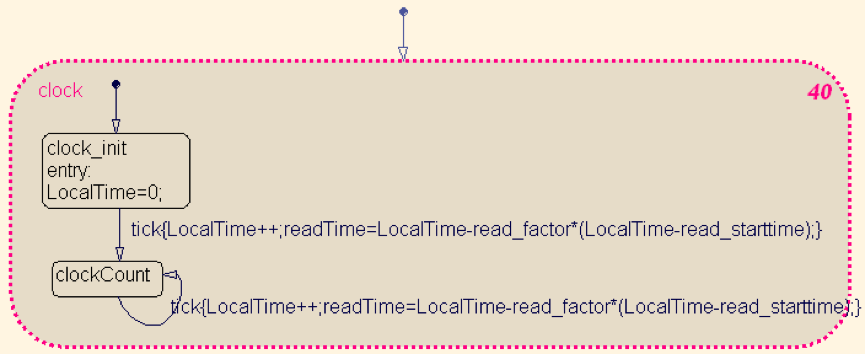
\includegraphics[width=12cm]{simulation_local_clock}
    \bicaption[fig:simulation_local_clock]{本地时钟仿真模型}{本地时钟仿真模型}{Fig}{The Simulation model of Local Clock}
  \end{minipage}     
\end{figure}

\subsubsection{定时器模块}
由于同步系统中存在很多中定时触发或超时事件,例如Sync报文的周期性发送,Announce报文的超时等待事件等。所以,添加了这个模块,为系统中所有周期性或有超时发生的事件进行触发。

下图是Announce超时事件定时器模块作为参考,其他定时器模块与之非常类似。
\begin{figure}[!hbp]
  \centering
  \begin{minipage}[b]{1\textwidth}
    \captionstyle{\centering}
    \centering
    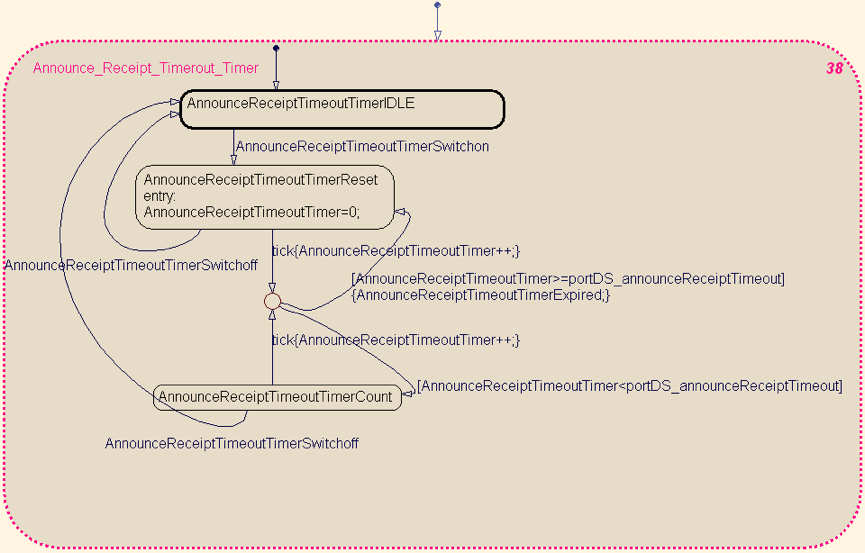
\includegraphics[width=12cm]{simulation_announce_timeout_timer}
    \bicaption[fig:simulation_announce_timeout_timer]{Announce报文超时事件定时器仿真模型}{Announce报文超时事件定时器仿真模型}{Fig}{The Timer model for Announce message receipt timeout}
  \end{minipage}     
\end{figure}

\subsubsection{报文收发模块}
该模块主要包括每个时钟内部对外的收发报文。对于接收模块,它会时钟监听某外部信号,一旦有报文传入则会立即触发系统进入报文接受流程,该流程会讲所收到报文的数据全部存储到本地,同时向系统中发出报文接受完成信号。对于发送模块,会先把数据根据对应报文格式组装成对应的报文,把数据存入该报文中,然后从时钟对应的端口发出。
\begin{figure}[!hbp]
  \centering
  \begin{minipage}[b]{1\textwidth}
    \captionstyle{\centering}
    \centering
    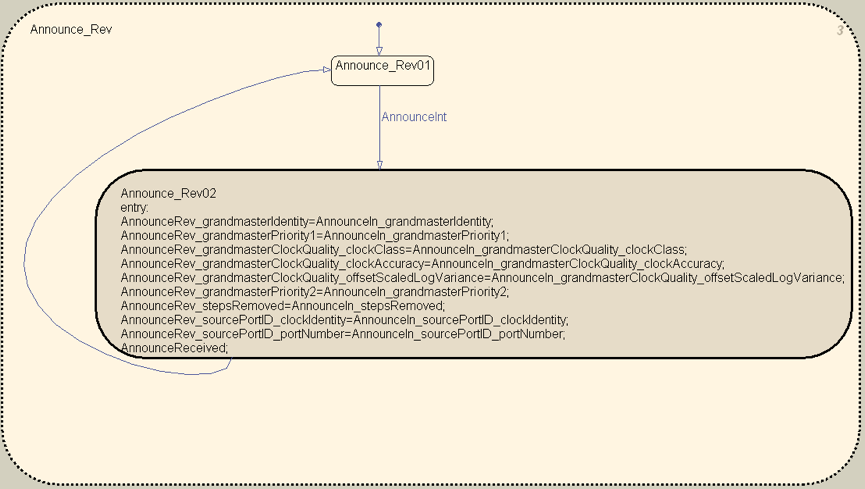
\includegraphics[width=12cm]{simulation_message_receive}
    \bicaption[fig:simulation_message_receive]{报文接收模块仿真模型}{报文接收模块仿真模型}{Fig}{The model for receiving message}
  \end{minipage}     
\end{figure}
\begin{figure}[!hbp]
  \centering
  \begin{minipage}[b]{1\textwidth}
    \captionstyle{\centering}
    \centering
    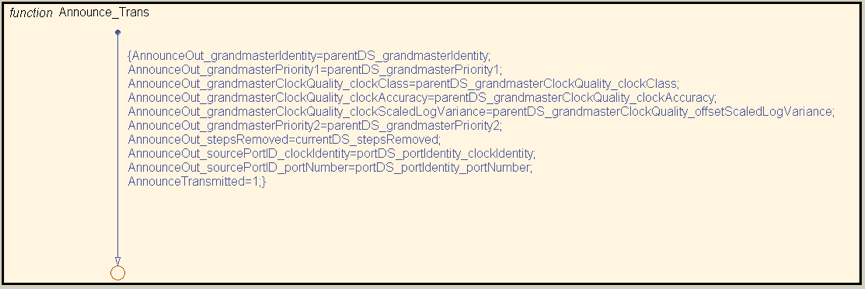
\includegraphics[width=12cm]{simulation_message_send}
    \bicaption[fig:simulation_message_send]{报文发送模块仿真模型}{报文发送模块仿真模型}{Fig}{The model for sending message}
  \end{minipage}     
\end{figure}

\subsection{算法仿真思路及指标分析}
下面,为了能够在stateflow仿真平台上验证上述所提统计算法的有效性,下面将从以下几个角度来进行模拟与验证。
\begin{itemize}[noitemsep,topsep=0pt,parsep=0pt,partopsep=0pt]
  \item 对于传输延时抖动,可以在传输中添加随机延时噪声来进行验证;
  \item 对于暂时性时延突变,可以对传输延时添加阶跃噪声,并观察对同步过程的影响;
  \item 对于持久性变化,可以在运行时链路传输中添加永久性固有延时,并观察结果;
  \item 对于控制策略,可以分别采取普通PI控制器校正和基于多模PID控制策略进行同步效果对比。
\end{itemize}

为了验证本文所提的优化算法,下面会在整个同步系统外部,通过监听主时钟和从时钟的时钟偏差曲线,从而可以知道该同步系统的同步性能。主要的比较指标有下面几点:
\begin{itemize}[noitemsep,topsep=0pt,parsep=0pt,partopsep=0pt]
  \item 偏差值:通过观察主从时钟的偏差值,可以看出该同步系统的同步效果,这也能直接反映真实的同步精度。因此,可以以此来检测同步系统中链路延时抖动和暂时性抖动对同步精度造成的影响。
  \item 鲁棒性:当系统中发生持久性时延变化,那么会造成从时钟发生较大的抖动,所以,可以依据此来检测针对持久性时延变化的优化算法的效果,如果该优化算法能够使的从时钟的抖动减小,那么表示从时钟的鲁棒性得到了提高。
  \item 收敛速度及稳定性:可以通过观察主从偏差的波动值,并计算其收敛时间。尤其是在链路环境发生变化,即类似工业环境中的多种复杂因素导致系统不稳定,以此来观察系统的收敛速度和最终的稳定性,从而来判断本文采用的基于多模型的PID控制器的效果。
\end{itemize}

\section{算法仿真及结果分析}
为了验证上文中提到的最小二乘线性回归算法,动态阈值法和实时动态监控算法的实际效果,下面一次对这三种算法进行验证。在验证中,可以通过认为模拟延时抖动、排队堵塞和拓扑结构变化等因素导致的时延变化,通过比较采用相关算法前后的同步曲线来得出相关结论。

下文中的同步曲线是指从时钟与主时钟之间的随时间变化的实时同步偏差曲线。

\subsection{验证最小二乘线性回归算法对延时抖动的优化}
为了验证最小二乘线性回归算法对延时抖动的优化效果,可以在从时钟计算链路传输延时时添加随机扰动,并模拟该扰动符合标准正态分布,得到下面两个仿真结果。见对比图\ref{fig:添加正态分布的随机抖动后的同步曲线}与\ref{fig:添加正态分布随机抖动且利用最小二乘处理后的同步曲线}。
首先,为了模拟生产环境中的随机噪声,在传输链路中加入服从正态分布的随机影响因子,然后进行同步,可以得到下面的同步曲线:
\begin{figure}[!hbp]
  \centering
  \begin{minipage}[b]{1\textwidth}
    \captionstyle{\centering}
    \centering
    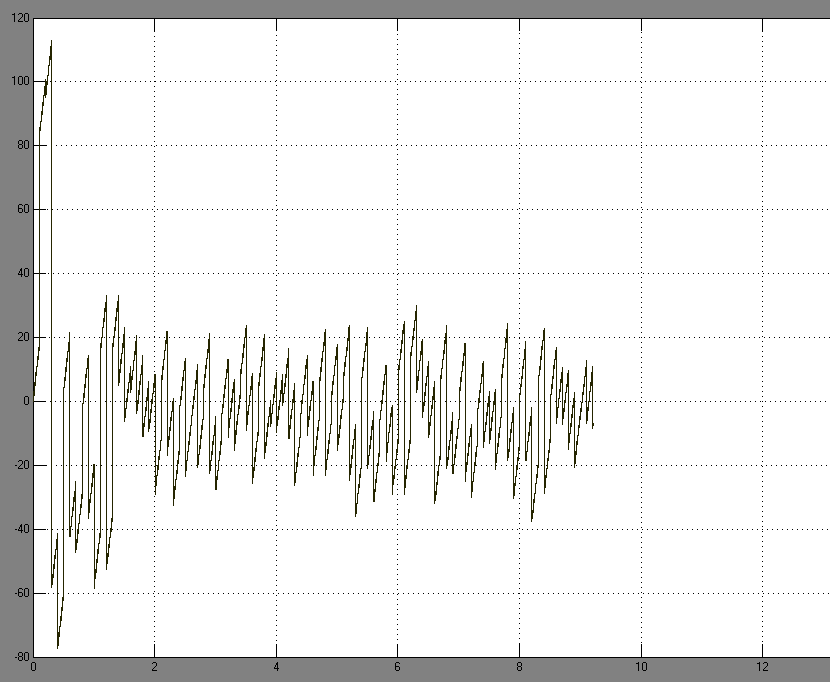
\includegraphics[width=8cm]{matlab/添加正态分布的随机抖动后的同步曲线.PNG}
    \bicaption[fig:添加正态分布的随机抖动后的同步曲线]{添加正态分布随机抖动的常规同步曲线}{添加正态分布随机抖动的常规同步曲线}{Fig}{The Synchronization curve, within Normal Distribution random noise}
  \end{minipage}     
\end{figure}

\begin{figure}[htbp]
  \centering
  \begin{minipage}[b]{1\textwidth}
    \captionstyle{\centering}
    \centering
    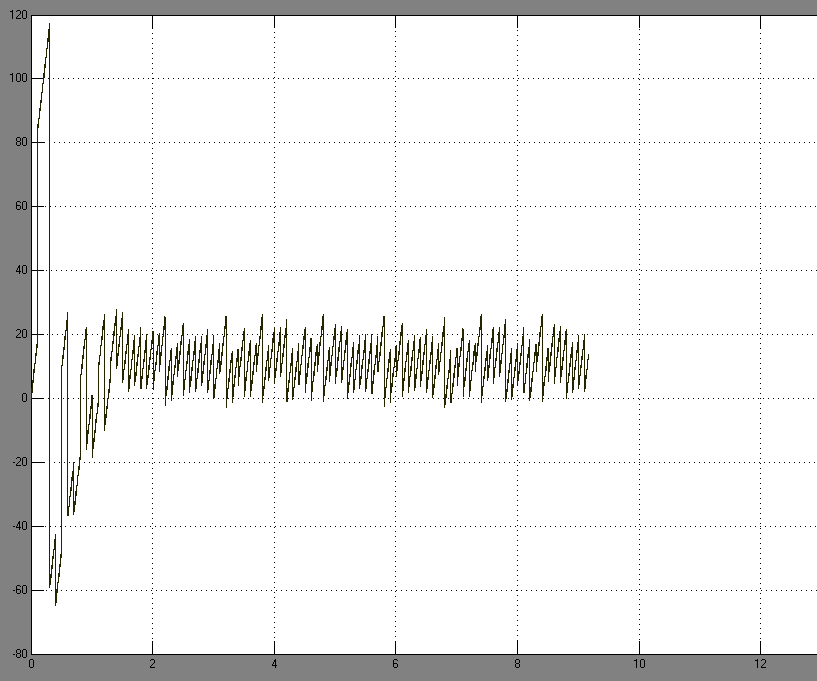
\includegraphics[width=8cm]{matlab/添加正态分布随机抖动且利用最小二乘处理后的同步曲线.PNG}
    \bicaption[fig:添加正态分布随机抖动且利用最小二乘处理后的同步曲线]{添加正态分布随机抖动且利用最小二乘处理后的同步曲线}{添加正态分布随机抖动且利用最小二乘处理后的同步曲线}{Fig}{The Synchronization curve dealing with least square method, within Normal Distribution random noise}
  \end{minipage}     
\end{figure}

通过上面的对比曲线,可以明显看出,利用最小二乘法处理后可以明显减小随机噪声对同步结果的影响,从时钟振动幅度减小,从时钟具有更好的同步效果。说明该线性回归算法能够很好的减小随机抖动对从时钟系统的影响。

\subsection{验证动态阈值法对暂时性时延突变的优化}
为了模拟暂时性时延变化,在同步系统运行中间,突然加入一个时延突变,并保持一小段时间。并分别仿真出采用动态阈值法前后的时钟同步曲线。见对比图\ref{fig:添加暂时性时延突变后的同步曲线}和\ref{fig:添加暂时性时延突变并采用动态阈值法处理后的同步曲线}。

首先,为了模拟暂时性时延突变,在仿真接近2秒时,为链路传输延时添加一个阶跃信号,并观察其同步曲线情况,可以得到如下结果:
\begin{figure}[htbp]
  \centering
  \begin{minipage}[b]{1\textwidth}
    \captionstyle{\centering}
    \centering
    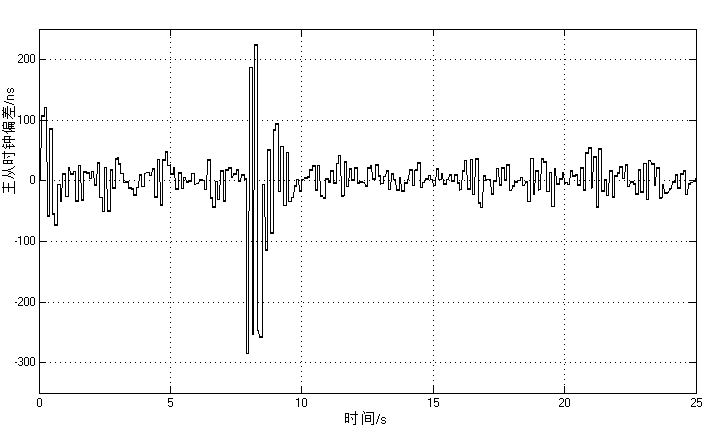
\includegraphics[width=9cm]{matlab/添加暂时性时延突变后的同步曲线.PNG}
    \bicaption[fig:添加暂时性时延突变后的同步曲线]{添加暂时性时延突变后的同步曲线}{添加暂时性时延突变后的同步曲线}{Fig}{The Synchronization curve, within temporary time-delay mutation}
  \end{minipage}     
\end{figure}

然后,保持上面的阶跃信号不变,采用文中采用的动态阈值法来进行优化,可以得到如下的结果如图\ref{fig:添加暂时性时延突变并采用动态阈值法处理后的同步曲线}。
\begin{figure}[!hbp]
  \centering
  \begin{minipage}[b]{1\textwidth}
    \captionstyle{\centering}
    \centering
    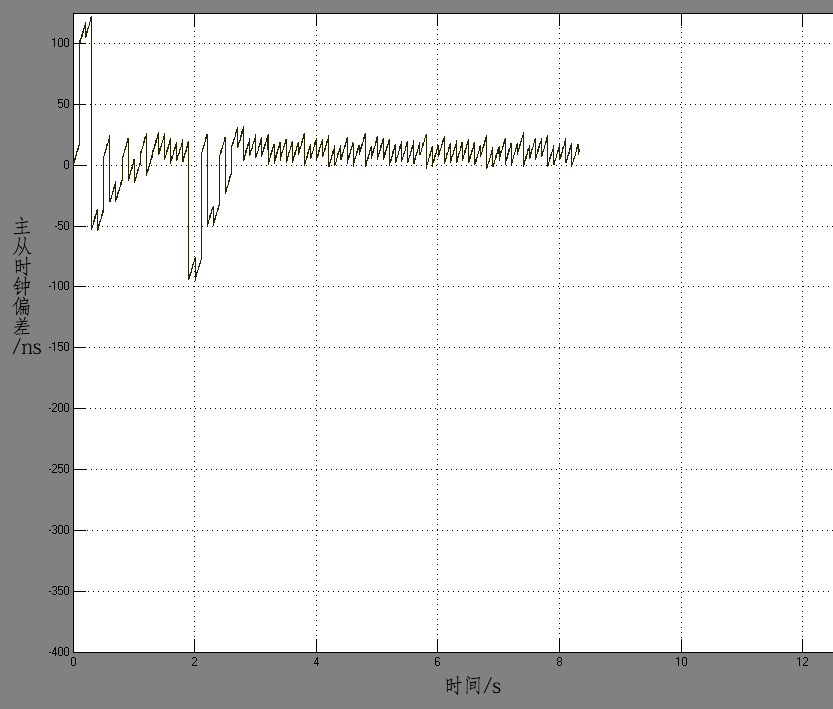
\includegraphics[width=9cm]{matlab/添加暂时性时延突变并采用动态阈值法处理后的同步曲线.PNG}
    \bicaption[fig:添加暂时性时延突变并采用动态阈值法处理后的同步曲线]{添加暂时性时延突变后,采用动态阈值法处理前后的同步曲线}{添加暂时性时延突变后,采用动态阈值法处理前后的同步曲线}{Fig}{The Synchronization curve with dynamic threshold value method, within temporary time-delay mutation}
  \end{minipage}     
\end{figure}

通过上面的对比曲线,可以明显看出,利用了动态阈值法对阶跃噪声进行优化后,从时钟的瞬间振荡明显减小,这意味着从时钟具备了更好的鲁棒性和稳定性,不会轻易随着网络负载变化而发生较大波动。

\subsection{验证实时动态监控算法对持久性时延变化的优化}
为了模拟持久性时延变化,在同步系统运行中间,加入一个恒定的时延变化,并保持不变。然后分别仿真出采用实时动态监控算法前后的时钟同步曲线。见对比图\ref{fig:添加持久性时延变化后样本逐步覆盖的同步曲线}与\ref{fig:添加持久性时延突变后,采用实时动态监控算法处理前后的同步曲线}。

为了模拟持久性延时变化,给链路延时添加固定的增量,并且保持不变,然后可以得到如下的同步曲线:

\begin{figure}[!hbp]
  \centering
  \begin{minipage}[b]{1\textwidth}
    \captionstyle{\centering}
    \centering
    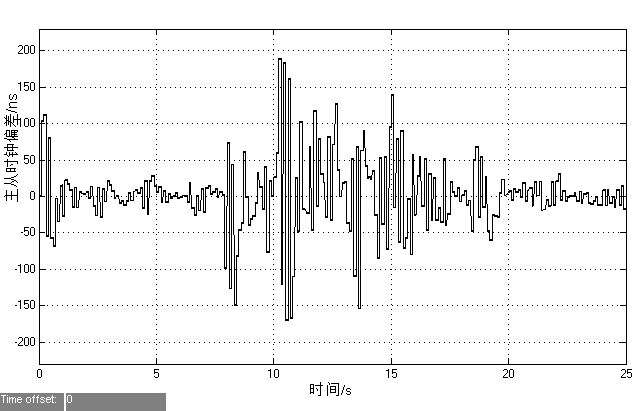
\includegraphics[width=9cm]{matlab/添加持久性时延变化后样本逐步覆盖的同步曲线.PNG}
    \bicaption[fig:添加持久性时延变化后样本逐步覆盖的同步曲线]{添加持久性时延变化后样本逐步覆盖的同步曲线}{添加持久性时延变化后样本逐步覆盖的同步曲线}{Fig}{The Synchronization curve, within persistence time-delay change}
  \end{minipage}     
\end{figure}

然后,保持上面的固定增量,采用动态监控方法来进行处理,可以得到同步曲线\ref{fig:添加持久性时延突变后,采用实时动态监控算法处理前后的同步曲线}。

\begin{figure}[htbp]
  \centering
  \begin{minipage}[b]{1\textwidth}
    \captionstyle{\centering}
    \centering
    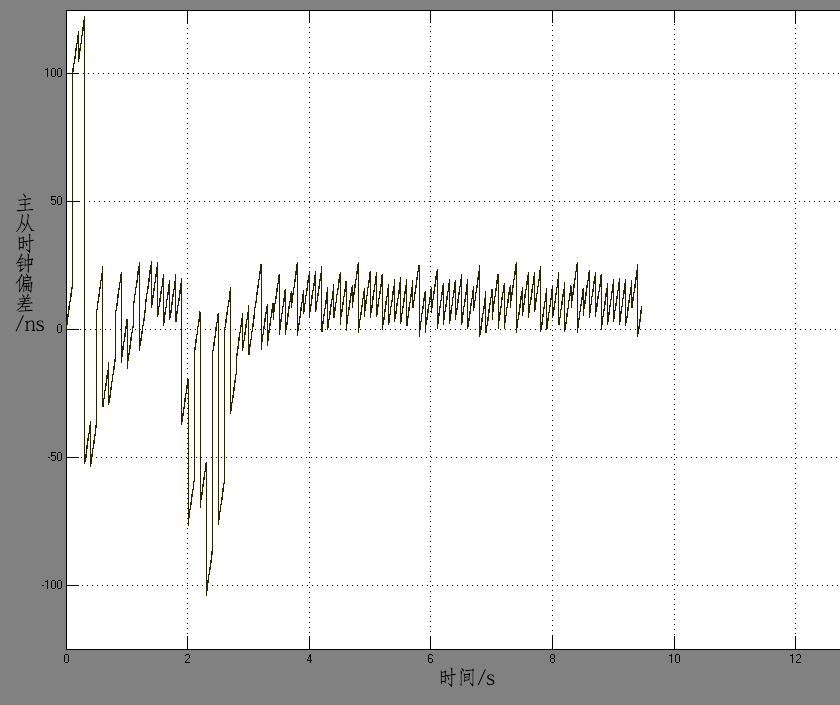
\includegraphics[width=10cm]{matlab/添加持久性时延变化后实时监控处理后的同步曲线.PNG}
    \bicaption[fig:添加持久性时延突变后,采用实时动态监控算法处理前后的同步曲线]{添加持久性时延变化后实时监控处理后的同步曲线}{添加持久性时延变化后实时监控处理后的同步曲线}{Fig}{The Synchronization curve with real-time dynamic monitoring method, within persistence time-delay change}
  \end{minipage}     
\end{figure}

可以发现,利用实时动态监控算法对持久性时延变化进行实时监控后,可以在系统中发生持久性时延变化后通过实时监控能够迅速发现该变化,然后采取相关措施后使得同步过程快速恢复正常,这提高了同步系统对外界变化的快速响应性。

\subsection{验证统计策略对晶振源频率补偿的优化效果}
为了在仿真系统中模拟从时钟晶振源漂移的情况,假设要模拟从时钟频率在不断衰减,即时间周期越来越长这样一种情况,那么可以给从时钟频率添加一个固定的衰减,使得从时钟的频率处于不断的小幅衰减中。然后,再利用上面采用的频率补偿算法,不断的对从时钟频率进行补偿,以保持主从时钟源频率尽可能的一致。

下面,先给从时钟源频率加上一个固定的衰减值,并观测主从时钟偏差的变化情况,可以得到同步曲线\ref{fig:为从时钟源频率添加固定衰减后的同步曲线}。
\begin{figure}[!hbp]
  \centering
  \begin{minipage}[b]{1\textwidth}
    \captionstyle{\centering}
    \centering
    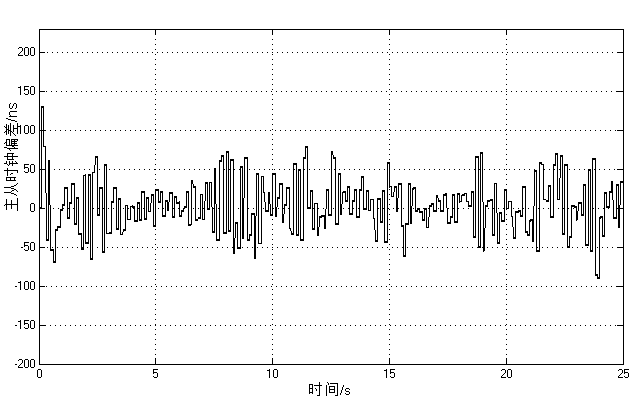
\includegraphics[width=10cm]{matlab/a默认晶振源漂移主从偏差.png}
    \bicaption[fig:为从时钟源频率添加固定衰减后的同步曲线]{为从时钟源频率添加固定衰减后的同步曲线}{为从时钟源频率添加固定衰减后的同步曲线}{Fig}{The Synchronization curve, within persistence time-decrease in slave clock}
  \end{minipage}     
\end{figure}

可以看出主从时钟源的偏差处于不断的波动之中。然后,为从时钟频率进行补偿,可以得到同步曲线\ref{fig:采用晶振源频率补偿算法后的同步曲线}。
\begin{figure}[htbp]
  \centering
  \begin{minipage}[b]{1\textwidth}
    \captionstyle{\centering}
    \centering
    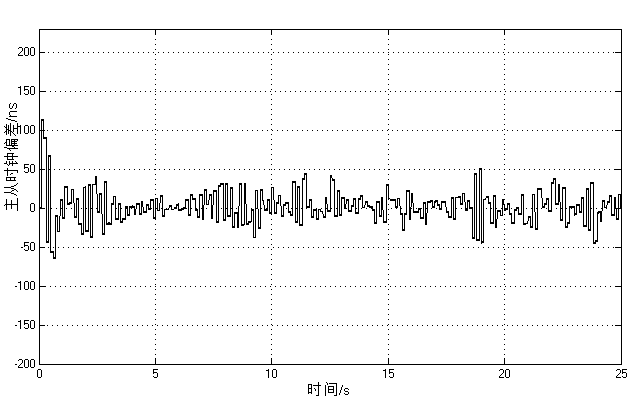
\includegraphics[width=10cm]{matlab/a晶振源漂移补偿后主从偏差.png}
    \bicaption[fig:采用晶振源频率补偿算法后的同步曲线]{采用晶振源频率补偿算法后的同步曲线}{采用晶振源频率补偿算法后的同步曲线}{Fig}{The Synchronization curve by frequency compensation, within persistence time-decrease in slave clock}
  \end{minipage}     
\end{figure}

通过上面的比较,可以看出,不使用频率补偿时,由于从时钟频率漂移导致主从时间差越来越大,需要校正的幅度也越来越大,所以会出现较大的波动。但是当对从时钟频率进行补偿后,使得主从时钟的频率更加接近,削弱了从时钟漂移带来的偏差,使得主从时钟同步的幅度减小,也更加的稳定。

\section{本章小结}
在本章节中,为了提高从时钟的稳定性,常规的做法是直接使用计算误差offset值对从时钟进行校正,不过那种做法会使得从时钟具有较大的波动,而且不能有效利用历史数据来进行调节。因此,本小结首先阐述了时钟伺服系统的概念,使用时钟伺服系统一般能够较好的提高同步系统的稳定性。然后,文中提到常规PID控制器校正,不过,为了应对延时阶跃性突变这种情况,文中又采用了一种多模型PID控制系统,即通过对控制误差进行检测,一旦发现控制误差发生阶跃变化,就切换控制器,以防止从时钟发生较大抖动,同时,在一定的观察时间段内,如果控制误差阶跃性恢复到原始值,则立即切换回常规PID控制,否则,直到观测时间短结束,才切回常规PID控制。阶跃信号会使得常规PID控制器控制后的从时钟发生频繁的调整,这会影响到依赖它的整个系统的抖动。而采用多模型PID控制系统可以把持续的波动转变成一个瞬时性的变化,这可以明显减小从时钟的频繁抖动,使整个系统更加稳定。

然后,对于常规的从时钟频率漂移补偿算法,一般都是通过记录一段时间内的Sync报文的发送和接收时间,以此来估算主时钟和从时钟各自的频率,并计算出二者的频率差来进行校正。这种做法没有本质错误,只是不能很好应对Sync报文在链路传输过程中发生的变化,一旦用来计算的Sync报文在传输时发生了较大的延时,那么从时钟处接收到的Sync报文就会滞后,从而导致频率计算出错。而本节中利用第三章中的统计算法,在从时钟处累计了一定Sync报文样本,可以先通过第三章的动态监测算法对报文进行过滤,即如果发现Sync报文发生了暂时性时延突变或者持久性时延变化,那么就丢弃当前时间段内的Sync报文,直到发现Sync报文传输较为稳定,才利用这些报文的收发时间来计算频率差。相对现有方法,它可以得到更加准确、不受外界因素影响的频率差。然后,为了适应新的ptp设备-透明时钟,文中首先对比了边界时钟与透明时钟的区别,然后将文中的多种统计算法依次进行调整,优化,使得这些统计方法能够更好的适用于透明时钟。最后,文中通过自己搭建基于stateflow的ptp仿真平台,对于文中采用的统计算法进行了仿真验证,通过最终的仿真结果可以看出统计算法不仅能够很好的提高同步系统对多种时延变化的鲁棒性,更能提高整个系统的同步精度和稳定性。

常规的时钟伺服系统一般采用PI或者PID控制器方法来进行从时钟控制,不过这种方法不能很好的处理链路延时发生阶跃性突变这种情况,因此,为了应对链路延时中发生的暂时性时延突变与持久性时延变化中触发的阶跃信号,文中采用的基于多模型PID控制系统,它会对校正残差进行突变监测,一旦发现阶跃变化,则立即切换控制器以确保从时钟的稳定性。相对现有方法,它能减小从时钟的频繁抖动,使的从时钟系统运行更加平稳。而且,由于常规的从时钟频率漂移补偿算法都是通过一段时间内的Sync报文来计算主从频率差,但并没有考虑到Sync报文在链路传输过程中发生的时延变化。而本文采用的动态监测算法会对报文进行过滤,只选取稳定传输下的Sync报文来进行计算,可以得到更加准确、不受外界因素影响的频率差。



